\section{パルサー研究の現状と未解決問題}\label{pulsar.s1}

パルサーに関する研究は天文学・宇宙物理学の広範囲にわたる。パルサーはそれ自体特異な天体であり、放射メカニズムや磁気圏の性質、進化など理解されていないことが多く、X線やガンマ線などの観測も利用してさかんに研究されている。一方でパルサーはその正確なパルス周期から、相対論の検証や重力波の検出にも用いられる。さらにrotation measureやdispersion measureなどを利用した銀河系構造の探索も行われている。SKAにより観測できるパルサーの数は飛躍的に増え、パルサー自体の研究もパルサーを道具として利用する研究も大きく進展すると期待される。この章ではパルサー研究の現状と未解決問題についてまとめる。


\subsection{パルサーの多様性}

パルサーは強い磁場($\sim 10^8-10^{14}$~G)を持ち高速に自転して($P\sim 10^{-3}-10$~sec)強い異方性を持った放射を出す中性子星である。中性子星の質量は太陽質量程度、半径は10km程度であり、超新星爆発の残骸として生まれると考えられている。またその形状は中性子の縮退圧と重力とのつりあいで保たれているが、中心付近の物理状態はまだ良く分かっていない。

\begin{figure}[t]
\centering
%\includegraphics[width=9cm]{pulsar/ppdotbin.eps}
\includegraphics[width=9cm,angle=270]{pulsar/ppdotdiagram.ps}
%\vspace{-0.5cm}
\caption{周期$P$とその時間微分$dP/dt$の平面におけるパルサーの分布\citep{Tauris15}。CCOはCentral Compact Object、XDINSはX-ray Dim Isolated Neutron Star、RRATはRotating Radio Transientである。星で囲まれているものは超新星残骸を伴っているもの、丸で囲まれているものは連星である。年齢一定と磁場一定の線も描かれている。}
\label{fig:ppdot}
\end{figure}

パルサーはこれまで2000個ほど見つかっているが、驚くほどの多様性を持っている。パルサーの多様性は、パルスの周期$P$とその時間変化$dP/dt$の平面での分布をみると分かりやすい(図\ref{fig:ppdot})。パルサーの年齢は典型的には$P^{-1}dP/dt$と見積もられ、パルサーの回転の減速が磁気双極子放射によると仮定すると磁場の強さは$\sqrt{P dP/dt}$に比例するのでこの図から年齢や磁場の強さの目安も得られる。ほとんどの通常のパルサーは周期が1秒あたりに分布しているが、そこから大きく離れているもの、変わった特徴を持つものがあるので以下まとめる。
\begin{itemize}
\item ミリ秒パルサー:$30~{\rm msec}$より短い周期を持つパルサーで図\ref{fig:ppdot}の左下に分布している。ほとんどは連星系をなしており、伴星からのガス降着によって回転が加速したと考えられている。これまで300個ほど見つかっており、その中でも周期が安定しているものは相対論の検証や重力波の直接検出に利用される。
\item マグネター:パルサーの中でも特に強い磁場($\sim 10^{14}~{\rm G}$)をもつパルサーである。ただしX線やガンマ線で発見されたものがほとんどで、電波放射が検出されているマグネターはごく一部である。
\item Central Compact Object (CCO):超新星残骸の中に熱的X線で見つかったパルサーであり、電波や可視光の対応天体は見つかっていない。またパルサー星雲も付随しておらず、まだパルサーとしての活動を始めていない中性子星であると考えられている。
\item Rotating Radio Transient (RRAT):散発的にしかパルサーとしての活動性を示さないパルサーであり、通常のパルサーよりやや長い周期を持つ。通常のパルサーがRRATに進化していくのかどうかはよくわかっていない。
\item Intermittent Pulsar:1か月に数日程度しか電波放射をしないパルサーである。しかも周期の時間変化を追っていくと、放射をしているときの方が放射をしていないときよりも回転速度の減速が大きくなっている。電波放射のエネルギーはパルサーの回転エネルギーの損失率よりもずっと小さいので、このような振る舞いは予想外で放射メカニズムに関する重要な示唆を与えていると考えられている。
\end{itemize}
以上のようにパルサーは多様であるが、その多様性がどこから来るのかが大きな問題になっている。特に中性子星が形成されたばかりのときにはどのような回転速度と磁場を持っているのか、その後これらがどう変化していくのかが中性子星の進化を探る上で重要である。


\subsection{パルサー磁気圏}

中性子星の磁気圏では、中性子星の持つ起電力によって、粒子が非常に高いエネルギーまで加速され、それに伴ってガンマ線から電波にわたる広帯域の放射や電子陽電子対生成が起こっていると考えられている。その中でも非常に輝度の高い電波パルスについては放射機構がまだ分かっていない。

粒子加速は磁力線に沿った電場によって起こっていると考えられており、その電場発生機構については従来、"Outer Gap"と"Polar Cap"という二つのモデルが提唱されて来た。"Outer Gap"モデルでは、中性子星の強い起電力に対してプラズマの供給が制限されているため、分極による電荷分離がはなはだしい中緯度地帯で粒子が枯渇し、結果として電場が形成されると考えている。一方、"Poler Cap"では磁力線に沿った電流の途中で磁力線電場をスクリーンする条件が満たされない領域が磁極上空に出来ると考える。粒子加速に"Outer Gap"と"Poler Cap"のどちらが効いているのか、あるいは両者とも共存しているのかは未解決問題である。

さらに最近、光円柱近傍の開いた磁場と閉じた磁場の境界領域での電流シートで粒子加速が起こるとする計算結果も出されており,パルサー磁気圏での粒子加速、電磁波放射機構の理解はまだ手探りの状態である。今後,すべての電磁波のチャンネルでより精密な観測を行い、電波放射の三次元構造を見る必要がある。

また、パルサーの回転エネルギーの殆どは、パルサー風と呼ばれる磁化したプラズマのoutflowによって運ばれている。パルサー風はパルサー周辺の物質と相互作用しパルサー星雲として観測されている。パルサー風のエネルギーを運ぶものが電磁場なのかプラズマの運動エネルギーなのか(パルサー風の加速効率)も、パルサー風の加速機構と同様になぞである。


\subsection{パルサーによる重力波検出}

1916年にアインシュタインによって提唱された一般相対性理論は重力を時空の歪みで表現し、さらにその歪みは波として伝搬することを予言した。この「重力波」の検出するために現在様々な実験が進められている。重力波の存在自体は1974年に連星パルサーPSR1913+16の軌道周期の減少から間接的に証明されたものの、直接検出は未だに達成されていない。これは重力が電磁気力に比べて相互作用する力が弱いことに起因する。しかし長期に渡って実験の改良が進められてきたことで、近年になってようやく検出が高い確率で期待される水準にまで感度が向上しつつある。

重力波は質量を持つ物体が加速度運動するときに放射され、大質量になるほどその強度が大きい。そのため、ブラックホール、中性子星、白色矮星といったコンパクト天体で構成される連星系や、超新星爆発などの劇的な現象が重力波観測の対象になる。放出される重力波の周波数はその現象のタイムスケールによって決まるため、質量が大きい物体ほど低周波の重力波を放出する。重力波が通過すると進行方向に対して垂直な面の空間の距離が伸び縮みするため、2点間の距離を非常に精密に測定することで重力波を検証することができる。

現在、重力波を直接検出するための実験で主に使われている方法はレーザー干渉計を用いる方法である。L字型に置かれたレーザー光で構成される干渉計を重力波が横切ると、空間の伸縮により光の到達時間が各方向によって異なるため干渉縞が生じる。この原理を使って重力波の検出を試みる実験は、神岡鉱山で建設が進む日本の重力波望遠鏡KAGRAの他に、アメリカのAdvanced-LIGOや欧州のAdvanced-VIRGOがあり、2017年前後の観測開始を予定している。これらの実験は周波数が約$100$Hzの重力波に対して最も良い感度を持ち、中性子星連星からの重力波を一年に10個程度は捉えられることが期待されている。

また、レーザー干渉計を使う方法とは全く異なり、宇宙観測を使って重力波を検証する方法も独立して並行に進められている。ひとつは宇宙マイクロ波背景放射のBモード偏光を観測する方法である。マイクロ波背景放射が放たれた時代に重力波が生み出す光子の偏光パターンを測定するため、宇宙のごく初期に生成された宇宙サイズの大きな波長の原始重力波を検証するのに有効である。さらにもうひとつの重力波検出実験として電波望遠鏡を使ったパルサータイミングがあり、SKAのメインサイエンスの一つである。

パルサータイミングの重力波検出の原理はレーザー干渉計と似ており、レーザーの代わりにミリ秒パルサーから正確な一定周期でやってくる電波パルスを用いる。重力波が通過する際に地球やパルサーの位置がずれることでパルスの周期が変化するため、異なる2方向のパルサーのパルス周期の変化を比べることで重力波を検証することができる。しかしこの重力波によるずれは非常に小さく、通常はパルサーが本来持つパルス間隔の不定性やパルスが伝搬する際に星間物質から受ける影響によるノイズに埋もれてしまう。そこで、重力波の空間の歪め方には方向に特徴的なパターンがあることを利用し、様々な方向にあるパルサーを複数観測して相関を取ることで重力波特有の歪みのパターンを取り出す方法が考えられている。この方法をパルサータイミングアレイと呼ばれる。ここで用いるパルサーはミリ秒パルサーで、その中でも特に周期の安定したものを選別する。

パルサータイミングアレイが感度を持つ重力波の周波数はパルサーを観測する頻度や観測を続ける期間によって決まり、典型的には$10^{-9}-10^{-8}$Hzである。このような周波数の重力波を放出するのは巨大ブラックホール連星で、銀河が衝突したときにそれぞれの銀河中心にあった巨大ブラックホールにより形成される。

これまでアメリカのNANOGrav、欧州のEPTA、オーストラリアのPPTAの3つのグループが各国の電波望遠鏡を使ってそれぞれ独自に重力波に対する上限を出してきた。それぞれの制限に大きな差はないが、一番厳しいものは$\Omega_{\rm GW}< 2.1\times 10^{-8}$で、現行のレーザー干渉計のLIGOとVIRGOによってつけられた制限$\Omega_{\rm GW}< 5.6\times 10^{-6}$より強い制限をつけている($\Omega_{\rm GW}$は宇宙のエネルギー密度に対する対数周波数あたりの重力波のスペクトル密度の割合)。また、現在はInternational Pulsar Timing Array (IPTA)として3グループが協力体制を築きながら、さらなる感度向上を目指して現在も観測を続けている。これまでの観測はすでに銀河衝突史の理論から予言される重力波の振幅の近くまで感度を伸ばしており、今後数年以内での検出が期待されている。

これに対してSKAによるパルサータイミングアレイでは利用するミリ秒パルサーの数を現行の30から100に増やし、パルス周期の測定のエラーを1/10程度に改善することで$\Omega_{\rm GW}\sim 10^{-13}$程度まで感度を伸ばすことができると見積もられている。このような高い感度を持つ実験で重力波の検出が可能になれば、重力波観測によって天文学に対して新たな知見がもたらされ、宇宙の成り立ちの理解を前進させるのに大きく役立つと期待される。



\subsection{パルサーによる一般相対論検証}

Ia型超新星の観測をはじめとして、様々な観測が現在の宇宙が加速膨張していることを裏付けている。宇宙の加速膨張を実現するためには、斥力的な重力相互作用を生み出す未知の暗黒エネルギーを導入するか、もしくは宇宙膨張を論じる上で前提となるアインシュタインの重力理論を修正する必要がある。他方、素粒子理論の究極の目標である全ての力(電磁力、弱い力、強い力、重力)の統一を目指すうえで、高エネルギー領域での重力理論の変更は避けられないと考えられている。このように、修正重力理論は観測・理論の両側面から興味を持たれている。

修正重力理論が我々の宇宙を記述しうる理論と位置付けられるためには、様々な検証をクリアする必要がある。まず第一に考えられるのは、我々の太陽系を記述するニュートンの逆二乗則の再現である。次に、ニュートン重力理論にアインシュタイン理論の補正を加えることで説明される水星の近日点移動などが考えられる。これらの重力理論の検証は、重力のふるまいがニュートン重力、もしくはそれからの小さな補正を用いて記述されるため、弱い重力場における検証と言われている。パルサーを用いた重力理論の検証は、それとは対極的に強い重力下での重力理論の検証を可能にする貴重な手段の一つである。

ここでパルサーを用いた強重力場における検証を行う意義は、それが弱い重力場における検証とは全く独立なものであることに加え、一般に重力の修正の効果は時空の曲率が大きくなるような場面によく現れる事が期待されるという点にある。つまり、パルサーを用いた検証を行うことにより、弱い重力場における検証に比べ、より強い制限が与えられることが期待できる。また他方で、弱い重力場の検証は、太陽系内の重力の振る舞いを検証しているにすぎないが、パルサーを用いることにより、太陽系外の重力の振る舞いを検証することが可能となる。宇宙の様々な場所の重力の振る舞いを確かめることは、重力理論の普遍性を検証する上で非常に重要である。以下では強い重力場における重力理論の検証について、その現状と可能性についてまとめる。

まず、パルサーによる重力理論の検証として最も有名なものは、ハルス・テーラー連星バイナリーを用いた重力波の存在の間接的証明が挙げられる。パルサーが他の星と連星系を成し、お互いの周りを回ると、パルス信号の到達時間は公転周期によって変調されるため、変調の観測から公転周期を測ることができる。一方、連星の加速度運動は重力波の放出を伴うことが一般相対性理論によって予言されている。重力波によって系からエネルギーが抜き取られると、そのエネルギーの減少に伴って軌道の公転周期が小さくなる。1974年に Hulse と Taylor によって初めて連星パルサーが発見され、その後の継続的な観測を経て、1979年にその公転周期の減少が確かなものとなった。他方、この観測された公転周期の減少率は、誤差の範囲で一般相対論の理論予想と一致し、これは重力波の存在を間接的ではあるが初めて捉えた観測、そして一般相対論の傍証を与えた観測であるとみなされている。
\begin{figure}[t]
\begin{center}
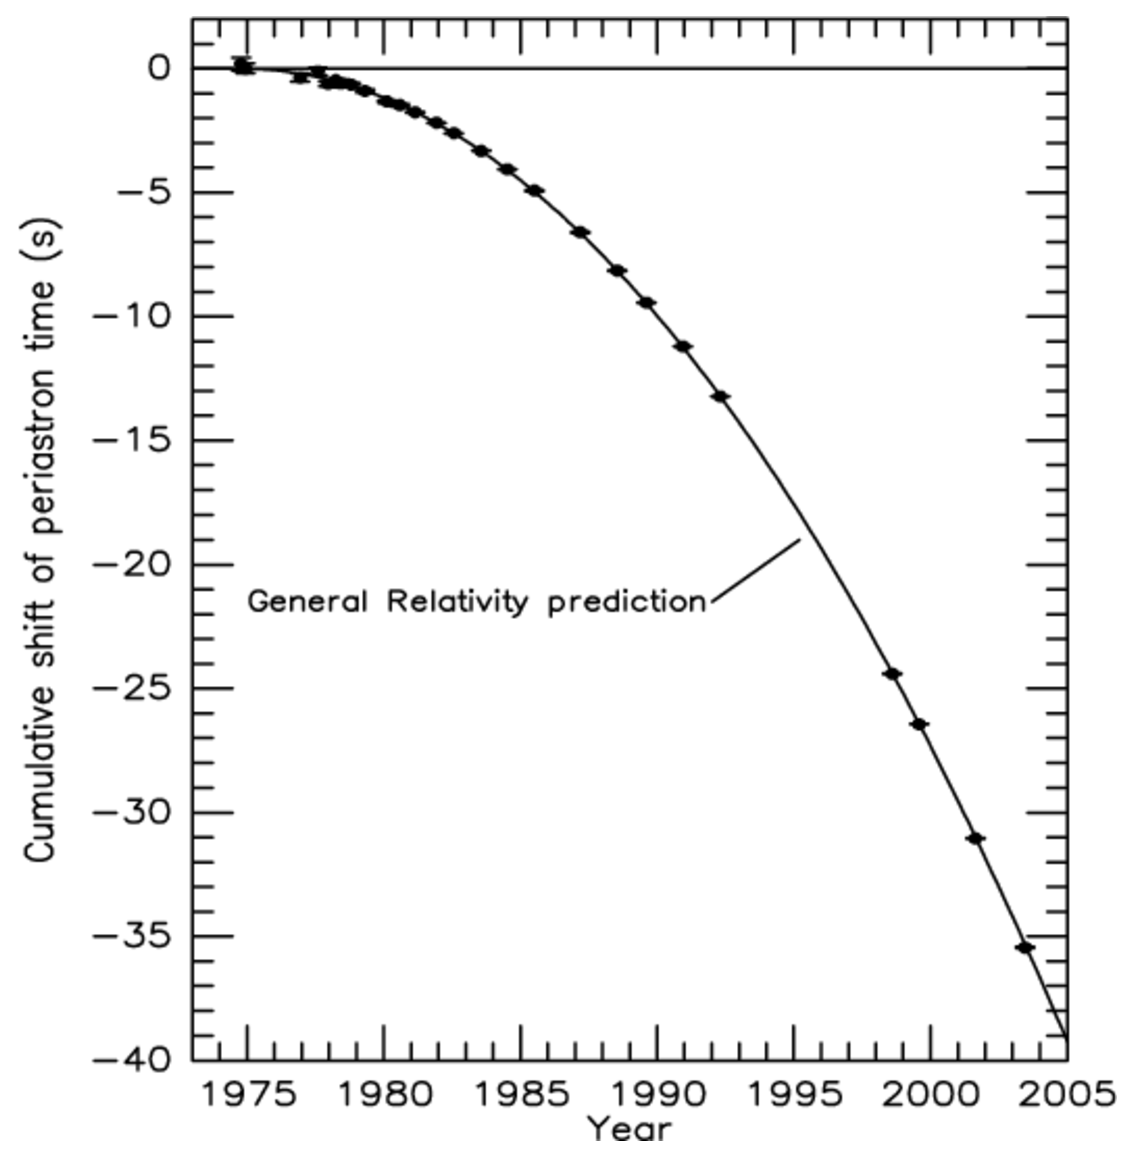
\includegraphics[width=80mm]{pulsar/binary_pulsar.eps}
\caption{
ハルス・テーラー連星バイナリーにおける公転周期の減少について、一般相対論に基づく理論曲線と観測結果。図は \cite{Weisberg:2004hi} から引用。
}
\label{fig_HT}
\end{center}
\end{figure}
重力波放出の詳細、例えば放出される重力波のエネルギー量などは修正重力の理論に依って一般に異なるため、同様の観測が多数の連星パルサーに対してより精密に行われれば,重力理論にこれまでにない強い制限が与えられるだろう。

次に、パルサーを用いたブラックホール周辺の重力場の検証について紹介する。ここではパルサーが銀河中心の巨大ブラックホールの周りを公転している状況を考えてみよう。パルサーから放出されるパルスの到達時間は、ブラックホール周りの重力場の影響を受ける。つまり、パルスにはブラックホール周りの重力場の情報が組み込まれることになり、この情報を通じてブラックホール時空の情報を直接的に抜き出すことが可能となる。一般相対論においてはブラックホールの無毛定理というものが存在し、定常軸対称で電荷をもたないブラックホールは、質量と角運動量 (スピン) という二つのパラメータのみで記述されることが知られている。それゆえ一般相対論によると、ブラックホール時空の全ての多極モーメントは、ブラックホールの質量とスピンを用いて完全に記述されることになる。パルスの情報から、質量や角運動量に加えて,多極モーメントを観測的に正確に抜き出すことができれば,それらの間の関係式、ひいてはそれを通じた重力理論の検証を行う事が可能となる。

以上のように、パルサーを用いた重力理論の検証は、太陽系における弱い重力場における重力のテストとは全く独立な、強い重力場における重力理論の検証を可能にするだけでなく、太陽系をこえて重力理論の普遍性を検証することを可能にし、他に類をみない非常に有意義な重力理論の検証の機会を与えてくれる。



\subsection{パルサーを用いた銀河系磁場構造探索}

ここでは銀河系磁場構造の観測的研究についてまとめる。

渦状銀河が大局的な磁場構造を持つことがシンクロトロン放射等から知られている。磁場強度は$\mu$Gのオーダーであり、エネルギー密度は星間空間のホットガスや宇宙線のエネルギー密度と同程度である.系外銀河の磁場構造はシンクロトロン放射の偏波やそのファラデー効果の観測から調べることができる。ファラデー効果は放射点から観測点までの伝播空間にある磁場により偏波角$\psi$が回転する現象であり、その効果はファラデー回転量(RM)で表される。
\begin{equation}
\psi = \psi_0 + \textrm{RM} ~ \lambda^2
\end{equation}
ここで$\psi_0$は電波源固有の偏波角、$\lambda$は電波の波長(m)である。ファラデー回転量RMは次式で表される,
\begin{equation}
\textrm{RM} = 0.81 \int_0^d n_e B_\parallel dl ~ [{\rm rad/m^2}]
\end{equation}
ここで,$d$は電波源までの距離(pc)、$n_e$は電子密度(cm$^{-3}$)、$B_\parallel$は磁場ベクトルの視線方向成分($\mu$G)である。ファラデー回転量の解析により,銀河磁場の大局構造には、軸対称(例えばM31)・非軸対称(例えばM51)の構造があることが予想されてきた。

我々の住む銀河系も渦状銀河と考えられている。その磁場構造については、系外電波源や系内のパルサーを電波源としたファラデー回転量を用いて調べることができる。ファラデー回転量の天球面上での分布を再現するように、磁場強度・方向・電子密度分布を求めるという方法である。銀河中心から8.5kpc程度に位置する太陽近傍については、銀河座標の銀経が約70-90度($l \sim 70^\circ$ - $90^\circ$)の方向へ太陽から離れる方向に磁場ベクトルが向いているとする結果が1970年代から得られている。

現在では,数万個の系外電波源でファラデー回転量が観測されている。例えばNVSS(NRAO VLA Sky Survey)による全天ファラデー回転マップがある\citep{TSS2009}。これらを用いた解析により、銀河系ハロー領域まで含めた広範囲の大局磁場構造について以下に述べるような結果が得られている.
\begin{itemize}
\item 銀河系円盤領域の磁場(円盤面に平行な成分)について、1)太陽近傍より外側では軸対称リング状の磁場構造、内側ではピッチ角を持ったスパイラル形の軸対称磁場構造、2)磁場の方向はNGP(North Galactic Pole)側から見て基本的に時計回り(銀河系中心を中心として)の方向を持つが、太陽より内側の領域で磁場の向きが反時計回りになる領域がある、という結果が得られている\citep{VE2011}。また、1 $\mu$G程度の大局磁場強度を得ている。
\item ハロー領域の磁場について、銀緯が高い位置($|b| \ge 10^{\circ}$)でのRMを用い,$b > 0^{\circ}$で反時計回り,$b < 0^{\circ}$で時計回りで,銀河面に対し反対称の結果を得ている\citep{PTKN2011}。
\item 銀河面に直交する方向の磁場成分について、$|b| \ge 77^{\circ}$のRMを用い,
NGP側ではRMの平均が$\langle \textrm{RM} \rangle \sim 0$ rad m$^{-2}$,SGP(South Galactic Pole)側で$\langle \textrm{RM} \rangle \sim +6.3$ rad m$^{-2}$という結果を得ている\citep{MAO2010}。これは,双極型や四重極型といった磁場モデルでは説明できない。
\item 銀河中心部について、$|l| < 6^\circ$, $|b| < 2^\circ$のRMを用い,銀河半径$r < 1$ kpcの範囲で,我々に向いた方向に,0.6 $\mu$G以上の強度の磁場があることが予測されている\citep{PPS2008}。この磁場構造は,銀河系中心部のbar構造に伴うものかもしれない.
\item 銀河系内に分布するパルサーのファラデー回転量を用いた解析では,よりこまかい磁場構造の議論ができる.例えば\cite{HAN2006}はスパイラルアームとインターアームに接する視線方向ごとにRMと視線距離の関係を調べた。そこから,銀河系の磁場構造は非軸対称的であり,アーム領域で反時計回り,インターアーム領域で時計回りの向きであることを予想している.
\end{itemize}
このように最近のファラデー回転量の解析は、
\begin{itemize}
\item ローカルアームより銀河中心側で磁場方向が反転していること
\item ハロー領域の磁場(円盤面平行成分)は銀河面反対称であること
\end{itemize}
を示している。観測データは増えているものの、RMの天球面分布にはデータのない領域もあり、銀河系大局磁場の決定には至っていない。また、ファラデー回転量に加え銀河系シンクロトロン電波の強度分布も同時に再現するよう磁場モデルを構築する研究も行われている\citep{SUN2008,JAFFE2010,JANSSON2012}。

また、銀河系の磁場・電子密度分布には乱流成分があり、これらのため観測されるRMは大きな分散を持ち大局磁場の決定に大きく影響している。電子密度の乱流成分については広い波長範囲でコルモゴロフ的であることが知られている\citep{ARM1995}。乱流磁場成分についても,RMを用いて研究されている。\cite{HBGM2008}はRMのstructure functionから、乱流磁場のインジェクションスケールを以下のように示した。
\begin{itemize}
\item アーム領域では,$l < 10$pcのスケール(星風などに対応)
\item インターアームでは$l \sim 100$pcのスケール(SNRなどに対応)
\end{itemize}
\cite{ARKG2013}はNGPとSGP方向の磁場構造について,系外電波源のRMを用いて議論した。大局磁場についてモデル磁場を用い、また乱流磁場にMHDシミュレーションの結果を用いて観測RMの再現を試みたが、観測RMの分布や統計的性質を説明することが困難であることを示している。これは、系外電波源のRMには電波源固有のRMや銀河間空間の寄与があること、また系内のローカルな構造の寄与が影響しているためかもしれない。観測されるRMには系内のHII領域などローカルな構造からの影響も大きいことが示されている\citep{MITRA2003,STS2011}。

\cite{OS1993}は幾何的に単純な大局磁場モデルを用いた解析では乱流磁場の評価が正しくできないことを指摘し、大局磁場モデルを利用せず乱流磁場を評価した。そして天球面で近接するパルサーペアについてファラデー回転量の差を用いた解析を行い、乱流磁場の強度が4-6 $\mu$Gと大局磁場強度($\sim 2 \mu$G)の数倍であることを示している。\cite{HAN2004}はこれを発展させて乱流磁場のパワースペクトルを評価した。その結果,0.5-15 kpcの波長域で$P(k) \propto k^{-0.37}$とコルモゴロフスペクトル($P(k) \propto k^{-5/3}$)よりフラットな結果を得ている。

大局磁場に加え,同等以上の強度を持つ乱流磁場成分から成る銀河系の磁場構造は星間プラズマの物理を考える上で重要である。また,高エネルギー宇宙線伝播への影響や系外電波への影響といった観点からも磁場構造を詳しく知ることが重要である。SKAにより、観測される系内外の電波源数が飛躍的に増えることや観測精度が向上することは、銀河系磁場構造のさらなる解明につながると期待される。



\subsection{Giant Radio Pulses}

パルサーからは周期的なパルス放射が観測される。その中でいくつかのパルサーでは、電波帯域において時折通常のパルス強度の数千倍~数百万倍にも達するGiant Radio Pulse (以下GRP)が観測される。約2000個のパルサーがこれまでに電波で見つかっているが\citep{Ma05}\footnote{``The ATNF Pulsar Database'', http://www.atnf.csiro.au/people/pulsar/psrcat/}、そのうちCrabパルサーや代表的なミリ秒パルサーであるPSR B1937+21など10個程度のパルサーでしかGRPの発見は報告されていない\citep{So04,RJ01}。

GRPに関しては、いくつかの理論モデルが提唱されているが\citep{Ly07}未だ解明には至っていない。しかし、例えば、CrabパルサーにおいてはGRPと可視光・X線・ガンマ線など他の波長帯のパルスとの相関について研究されている。GRPと同時発生した可視光帯域のパルスには$\sim 3\%$の有意な増光が見られている\citep{Sh03,St13}。より高いエネルギーではまだ統計的に有意でないものの、可視光と同程度の制限まで迫りつつある\citep{Mi14}。可視光より高いエネルギーの放射機構については比較的理解が進んでいるため\citep{Ta07}、それらとの相関関係を明らかにすることで、GRPを伴う現象の理解が今後飛躍的に進む可能性がある。

さらに、CrabパルサーのGRPではナノ秒オーダーでの激しい強度変動が観測されている\citep{Ha03,Ha07}(図\ref{nano}参照)。
\begin{figure}[t]
\centering
\includegraphics[width=11cm]{pulsar/nanoshot2.epsi}
\caption{8-10GHz帯で観測されたCrabパルサーのGRP\citep{Ha07}。ナノ秒オーダーの激しい強度変動(``nanoshot'')が見られ、ピークでは0.4ナノ秒間に2MJyを超えるフラックス密度が観測された。}
\label{nano}
\end{figure}%
ナノ秒オーダーの強度変動は、放射源の空間的スケールが数十cmであることを示唆する。超高時間分解能の観測により、数千光年離れた天体における数十cmの放射源を「分解」できた意義は非常に大きい。第一原理に近い数値シミュレーションによる検証も進みつつあり\citep{Ti12}、観測・理論両面において今後の研究発展が大いに期待される課題である。

